%****************************************************************
% Chapter X
%****************************************************************
\label{chapter-implementation}
\chapter{Implementation}

%****************************************************************
\section{Google VR SDK}

****************************************************************\\%####

%****************************************************************
\section{OpenGL ES}

****************************************************************\\%####
Pass Perspective matrix, View matrix, and Model matrix to shader to avoid calculate MV or MVP in cpu\\
Perspective: eye.getPerspective(float zNear, float zFar)\\
View: eye.getEyeView() * camera.matrix\\
camera.matrix: build by position, lookAt, up\\
Model: translation * scale * rotation * mat(1)\\

%****************************************************************
\section{File Server}

****************************************************************\\%####
Web server - golang - https://golang.org/pkg/net/http/\\
http.FileServer\\
https://github.com/ant0ine/go-json-rest\\
Go-Json-Rest is a thin layer ("Keep it simple, stupid") on top of net/http that helps building RESTful JSON APIs easily.\\
Volley - an HTTP library that makes networking for Android apps easier and most importantly, faster.\\
https://developer.android.com/training/volley/index.html\\

%****************************************************************
\subsection{Assets}

****************************************************************\\%####
static, layer, kml, resource,model\\

%****************************************************************
\subsection{Patch}

%****************************************************************
\section{Scene}

****************************************************************\\%####

%****************************************************************
\subsection{Keyhole Markup Language}

In this project, we only take use of few feature of KML \ref{fig:kml-schema}: Container, Style, Placemark,  and NetworkLink. The KML parser we are using is based on the open-source library \code{android-maps-utils} \parencite{Google.code-kml.2016} (NetworkLink is one of the unsupported feature in the library). Main modifications are getting rid of \code{com.google.android.gms.maps.GoogleMap} dependency, and extending \code{NetworkLink} feature support in accordance with the current design pattern.

\begin{figure}[H]
\caption[kml-parser-simple]{kML parser simple}
\label{fig:kml-parser-simple}
\centering
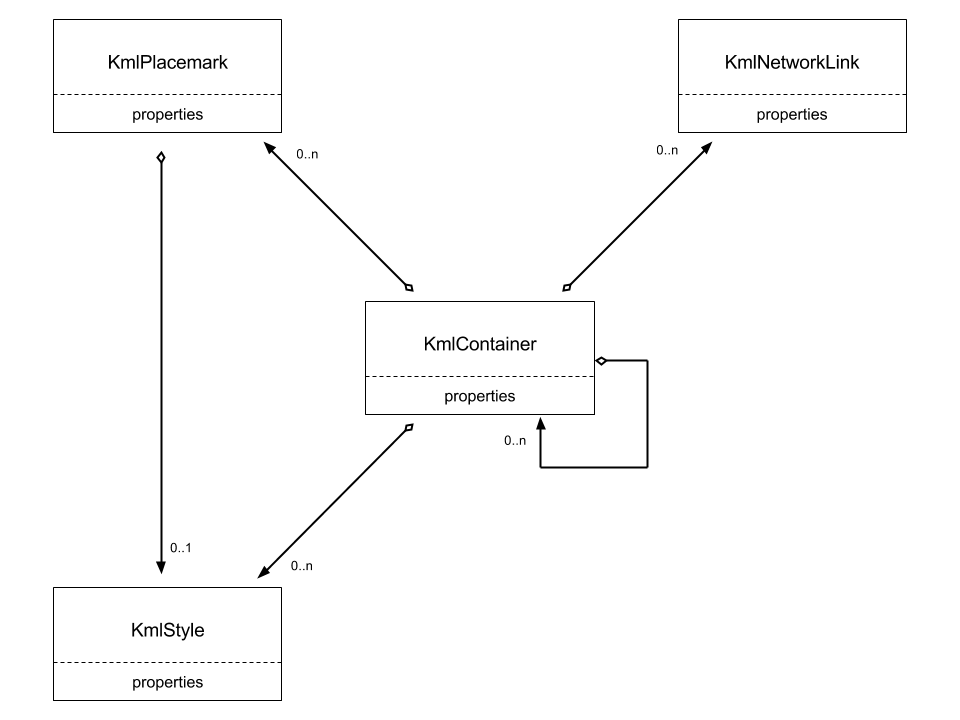
\includegraphics[width=\linewidth]{Figures/kml-parser-simple.png}
\decoRule
\end{figure}

%****************************************************************
\subsection{Octree} 
\label{section:octree}

To reduce the ray-object intersection tests,  space partitioning is needed. The main requirement is not to use a spatial data structure for an ray intersect with irregular geometry, but to determine what objects are in the same cell to avoid doing an $n^2$ check on all objects. In this case, it is spherical placemark. Therefore, we don't need overlapped volumes, and contained objects don't need to be cut on volume boundaries. It is actually 3D space partitioning process with a predefined restricted maximum number of objects in the same cell. A simple axis-aligned Octree is fully satisfy in here \ref{fig:octree-split}.

\begin{figure}[H]
\caption[octree-split]{Octree split}
\label{fig:octree-split}
\centering
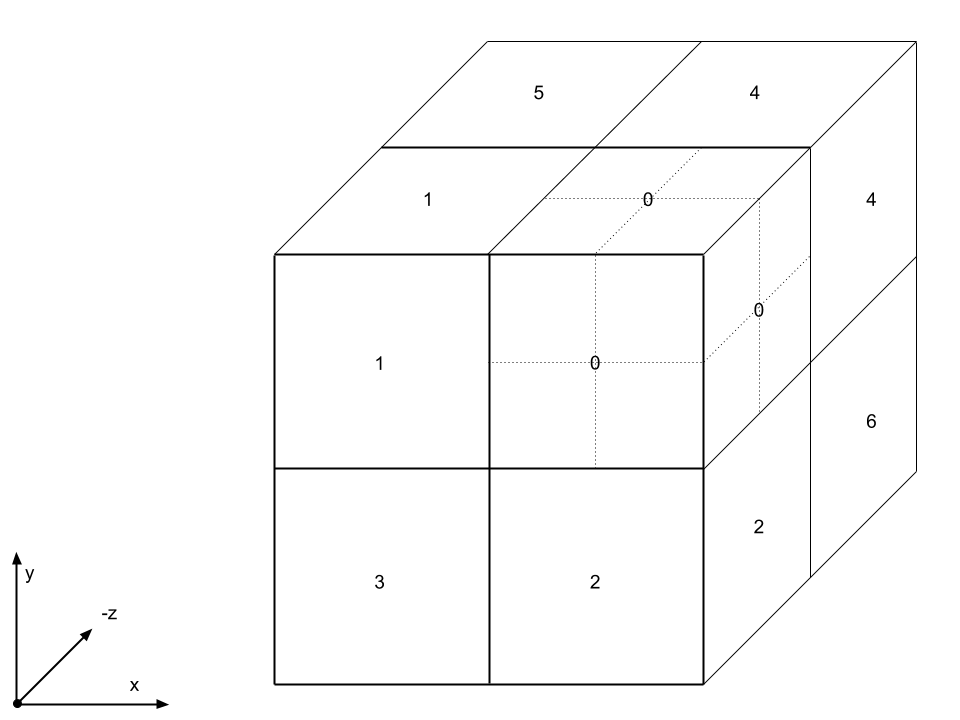
\includegraphics[width=\linewidth]{Figures/octree-split.png}
\decoRule
\end{figure}

For each box splitting process, we also generate eight indexes to indicate the relative position inside the box. These indexes are importent for the next partition, where we might need to relink contained objects to the new corresponding box. To insert a object into
the box only if the existed contained number of objects is less then the predefined constant value, otherwise splitting the box then relink existed object and insert the new object again.

Integer indexes of box is defined by three boolean valuse that indicates three axis-relative value:

Any position\;\emph{P} in the box with known center\emph{O}:

\[
\begin{array}{lr}
\begin{aligned}
dx &= P_x - O_x\\
dy &= P_y - O_y\\
dz &= P_z - O_z\\
\end{aligned}
\end{array}
\]

\begin{table}[H]
\caption{Octree Octant}
\label{tab:octree-octant}
\centering
\begin{tabular}{l l l l}
\toprule
\tabhead{Index} & \tabhead{Octant} & \tabhead{Geometric Meaning}\\
\midrule
0x00000000 & T,\;T,\;T & dx > 0, dy > 0, dz > 0\\
0x00000001 & F,\;T,\;T & dx < 0, dy > 0, dz > 0\\
0x00000010 & T,\;F,\;T & dx > 0, dy < 0, dz > 0\\
0x00000011 & F,\;F,\;T & dx < 0, dy < 0, dz > 0\\
0x00000100 & T,\;T,\;F & dx > 0, dy > 0, dz < 0\\
0x00000101 & F,\;T,\;F & dx < 0, dy > 0, dz < 0\\
0x00000110 & T,\;F,\;F & dx > 0, dy < 0, dz > 0\\
0x00000111 & F,\;F,\;F & dx < 0, dy < 0, dz < 0\\
\bottomrule
\end{tabular}
\end{table}

Octant solution:
\[
\code{octant[] = (index \& 1, index \& 2, index \& 4)}
\]

Index solution:
\[
\begin{array}{lr}
\begin{aligned}
\code{For Each oction[i]:}&\\
&\code{index |= (1 < < i)}\\
\end{aligned}
\end{array}
\]

%****************************************************************
\section{Earth}

The Earth is created as a UV Sphere, which somewhat like latitude and longitude lines of the earth, uses rings and segments. Near the poles (both on the Z-axis with the default orientation) the vertical segments converge on the poles. UV spheres are best used in situations where you require a very smooth, symmetrical surface.

\begin{figure}[H]
\caption[uv-sphere-mapping]{UV sphere mapping}
\label{fig:uv-sphere-mapping}
\centering
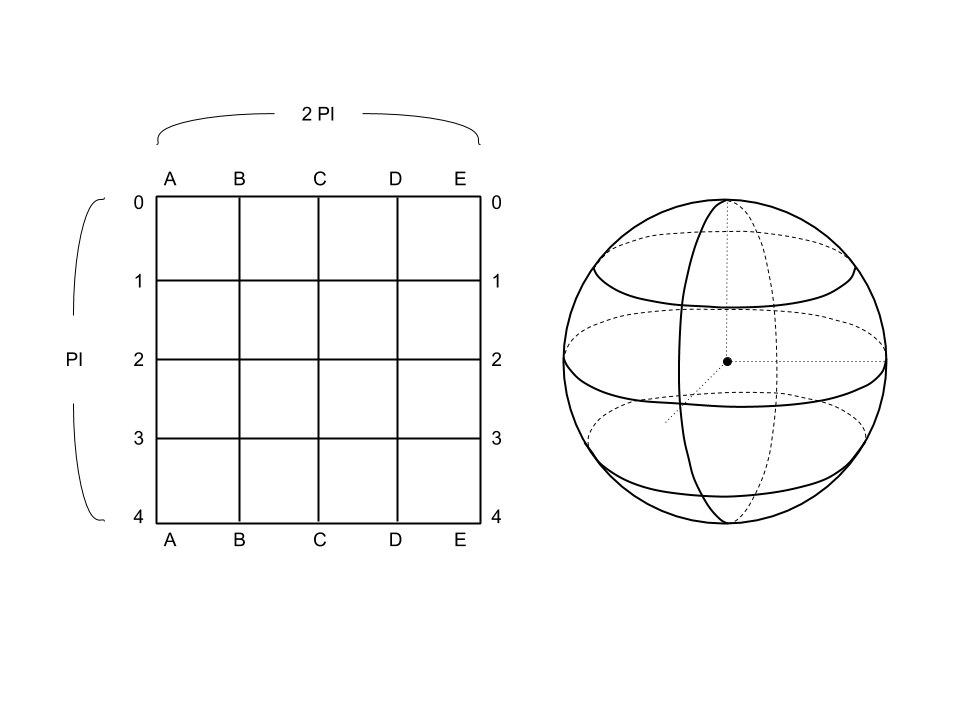
\includegraphics[width=\linewidth]{Figures/uv-sphere-mapping.png}
\decoRule
\end{figure}

As we can see the mapping from \ref{fig:uv-sphere-mapping}. Vertex $A0,\;A1,\;A2,\;A3,\;A4$ and $E0,\;E1,\;E2,\;E3,\;E4$ are duplicated, and $A0,\;B0,\;C0,\;D0,\;E0$ converge together as well as $A4,\;B4,\;C4,\;D4,\;E4$. So we can simply define it as a UV sphere has 5 rings and 4 segments. Also be noticed that each ring spans $2\,\pi$ radians, but each segment spans $\pi$ radians in the sphere mapping.

The total vertex number is:

\begin{equation}
\label{equ:uv-sphere-vertices}
Vertices = Rings \times Segments
\end{equation}

\begin{figure}[H]
\caption[uv-sphere-vertex]{UV sphere vertex}
\label{fig:uv-sphere-vertex}
\centering
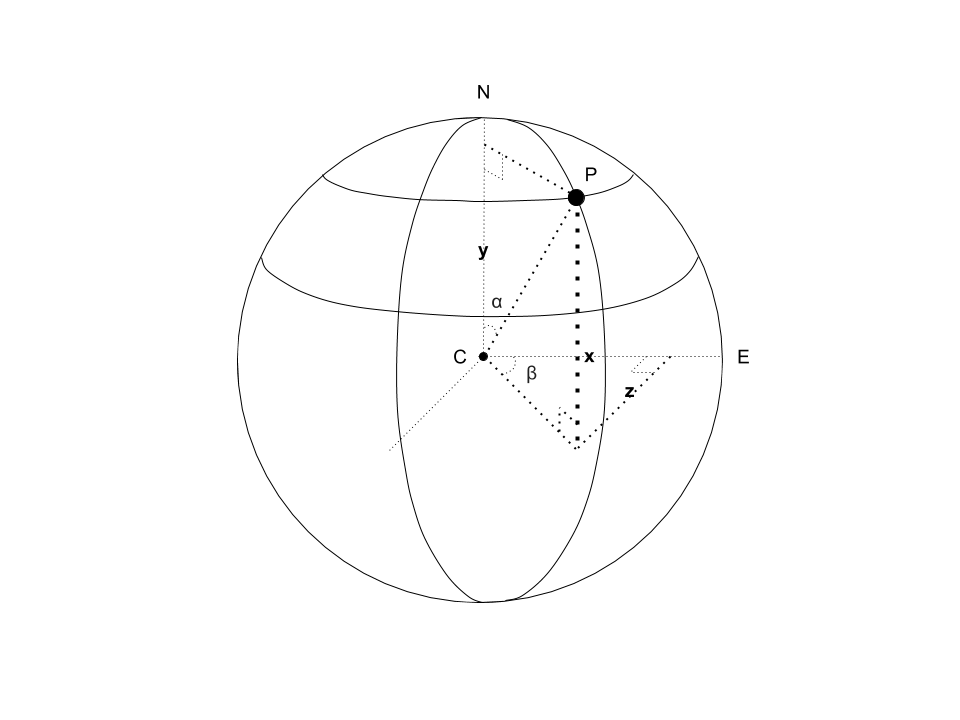
\includegraphics[width=\linewidth]{Figures/uv-sphere-vertex.png}
\decoRule
\end{figure}

For each vertex $P$ on sphere from ring $r$ and segment $s$, we have:

\[
\begin{array}{lr}
v = r \times  \frac{1}{rings - 1}\\
u = s \times  \frac{1}{segments - 1}\\
\measuredangle \alpha = v \times \pi\\
\measuredangle \beta = u \times 2\,\pi\\
\end{array}
\]

$\therefore$ P (x,\;y,\;z)
\[
\begin{array}{lr}
x = (\sin(\alpha) \times radius) \times \cos(\beta)\\
y = \cos(\alpha) \times radius\\
z =  (\sin(\alpha) \times radius) \times \sin(\beta)\\
\end{array}
\]

$\And$ 2D Texture (x,\;y) mapping for vertex $P$ is:
\[
\begin{array}{lr}
x = u\\
y = v\\
\end{array}
\]

%****************************************************************
\section{Placemarker}

Generation of vertices for placemarker is a recursion process of subdividing icosphere. Figure \ref{fig:icosahedron-rectangles} shows that the initial vertices of an icosahedron are the corners of three orthogonal rectangles.

\begin{figure}[H]
\caption[icosahedron-rectangles]{Icosahedron rectangles \parencite{wiki.icosahedron-rectangles.2006}}
\label{fig:icosahedron-rectangles}
\centering
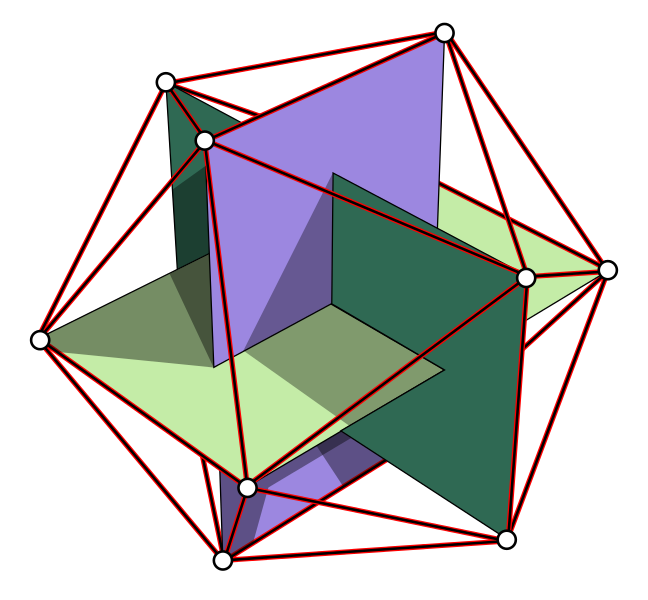
\includegraphics[width=\linewidth]{Figures/icosahedron-rectangles.png}
\decoRule
\end{figure}

Rounding icosphere by subdividing a face to an arbitrary level of resolution. One face can be subdivided into four by connecting each edge's midpoint.

\begin{figure}[H]
\centering
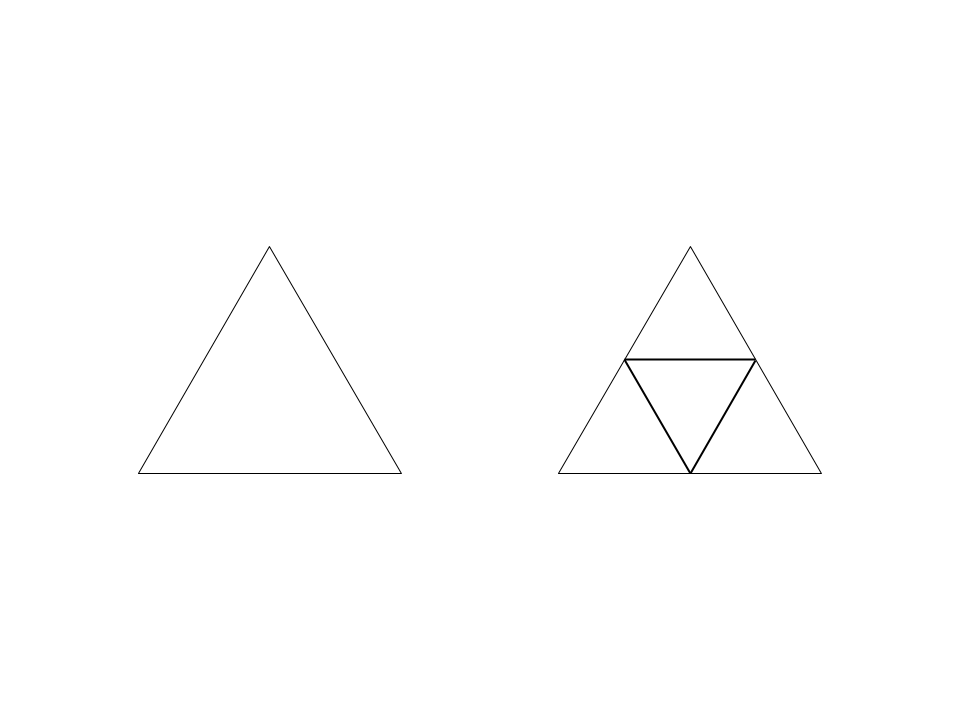
\includegraphics[width=\linewidth]{Figures/icosphere-subdivide.png}
\decoRule
\caption[icosphere-subdivide]{Icosphere subdivide}
\end{figure}

Then, push edge's midpoints to surface of the sphere.

\begin{figure}[H]
\centering
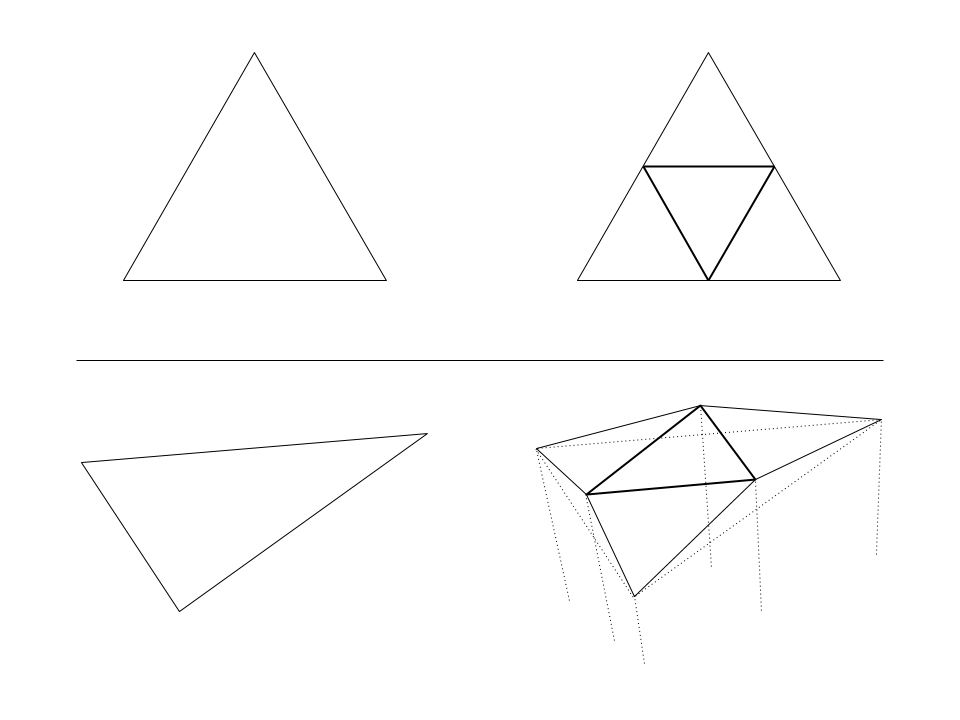
\includegraphics[width=\linewidth]{Figures/icosphere-refinement.png}
\decoRule
\caption[icosphere-refinement]{Icosphere refinement}
\end{figure}

\begin{table}[H]
\caption{Rounding Icosphere}
\label{tab:rounding-icosphere}
\centering
\begin{tabular}{l l l l}
\toprule
\tabhead{Recursion Level} & \tabhead{Vertex Count} & \tabhead{Face Count} & \tabhead{Edge Count}\\
\midrule
0 & 12 & 20 & 30\\
1 & 42 & 80 & 120\\
2 & 162 & 320 & 480\\
3 & 642 & 1280 & 1920\\
\bottomrule
\end{tabular}
\end{table}

%****************************************************************
\subsection{Geographic Coordinate System}

A geographic coordinate system is a coordinate system that enables every location on the Earth to be specified by a set of numbers or letters, or symbols \parencite{wiki.geographic-coordinate-system.2016}. A common geodetic-mapping coordinates is latitude, longitude and altitude (LLA), which also is the raw location data read from KML.

We introduce ECEF ("earth-centered, earth-fixed") coordinate system for converting  LLA coordinates to position coordinates. According to, the z-axis is pointing towards the north but it does not coincide exactly with the instantaneous earth rotational axis. The x-axis intersects the sphere of the earth at $0$ latitude and $0$ longitude \parencite{wiki.ecef.2016}.

\begin{figure}[H]
\centering
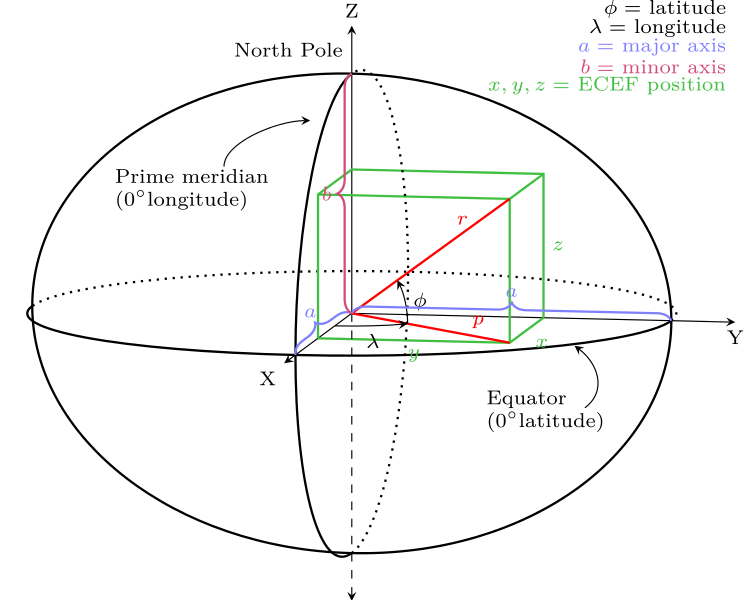
\includegraphics[width=\linewidth]{Figures/ecef.png}
\decoRule
\caption[ecef]{earth-centered, earth-fixed \parencite{wiki.ecef.2016}}
\end{figure}

The ECEF coordinates are expressed in a reference system that is related to mapping representations. Because the earth has a complex shape, a simple, yet accurate, method to approximate the earth’s shape is required. The use of a reference ellipsoid allows for the conversion between ECEF and LLA \parencite{u-blox.datum.1999}.

A reference ellipsoid can be described by a series of parameters that define its shape and which include a semi-major axis ($a$), a semi-minor axis ($b$), its first eccentricity ($e_1$) and its second eccentricity ($e_2$) as shown in Table \ref{tab:WGS-84-parameters}.

\begin{table}[H]
\caption{WGS 84 parameters}
\label{tab:WGS-84-parameters}
\centering
\begin{tabular}{l l l}
\toprule
\tabhead{Parameter} & \tabhead{Notation} & \tabhead{Value}\\
\midrule
Reciprocal of flattening & $1 / f$ & 298.257\,223\,563\\
Semi-major axis & $a$ & 6\,378\,137\,m\\
Semi-minor axis & $b$ & $a\,(1 - f)$\\
First eccentricity squared & $e_1^2$ & $1 - b^2 / a^2 = 2\,f - f^2$\\
Second eccentricity squared & $e_2^2$ & $a^2 / b^2 - 1 = f\,(2 - f) / (1 - f)^2$\\
\bottomrule
\end{tabular}
\end{table}

\begin{figure}[H]
\centering
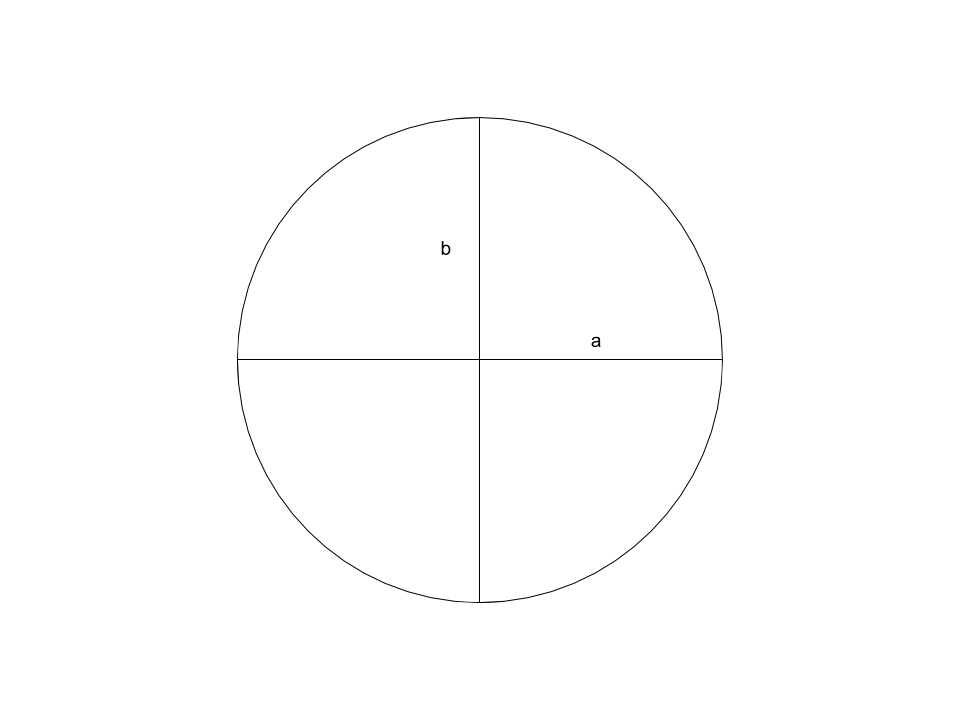
\includegraphics[width=\linewidth]{Figures/ellipsoid-parameters.png}
\decoRule
\caption[ellipsoid-parameters]{Ellipsoid Parameters}
\end{figure}

The conversion from LLA to ECEF is shown below.

\begin{figure}[H]
\centering
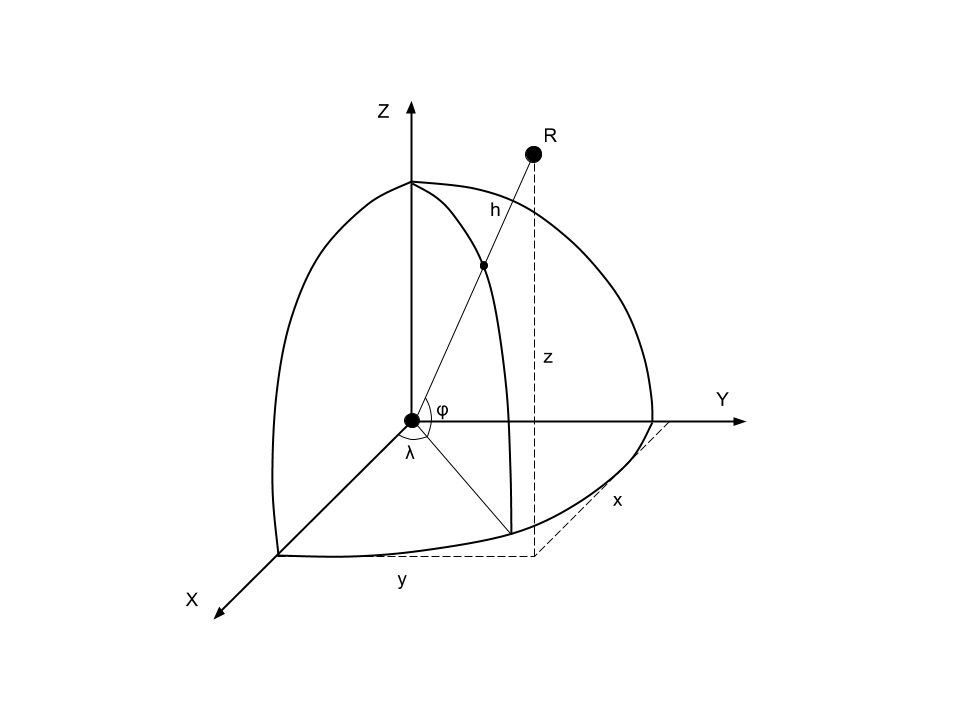
\includegraphics[width=\linewidth]{Figures/lla2ecef.png}
\decoRule
\caption[lla2ecef]{LLA to ECEF}
\end{figure}

\[
\begin{array}{lr}
\begin{aligned}
x &= (N + h)\,\cos(\varphi)\,\cos(\lambda)\\
y &= (N + h)\,\cos(\varphi)\,\sin(\lambda)\\
z &= (\frac{b^2}{a^2}\,N + h)\,\sin(\varphi)\\
\end{aligned}
\end{array}
\]

Where

\[
\begin{array}{lr}
\begin{aligned}
\varphi &= \text{latitude}\\
\lambda &= \text{longitude}\\
h &= \text{height above ellipsoid (meters)}\\
N &= \text{Radius of Curvature (meters), defined as:}\\
&= \frac{a}{\sqrt{1 - e^2\,\sin(\varphi)^2}}\\
\end{aligned}
\end{array}
\]

At last, for this project usage, where high accuracy is not required, $a$ equals to $b$. And also the ECEF coordinate system is y-east, z-north (up), and x points to $0$ latitude and $0$ longitude, but for project specific, we still need to convert ECEF to x-east, y-north (up), and x points to $0$ latitude and $180$ longitude.

%****************************************************************
\subsection{Description}

Description of placemarker requires an appropriate analysis for display. The raw data of description is a set of characters that could be a normal text, an image URL, an URL returns different type of content, or maybe just some meaningless characters.

Althrough the implementation of analysis in this project did not cover every situation, but it is flexible and extendable for more functionality.

\begin{figure}[H]
\caption[description-analysis]{Description Analysis}
\label{fig:description-analysis}
\centering
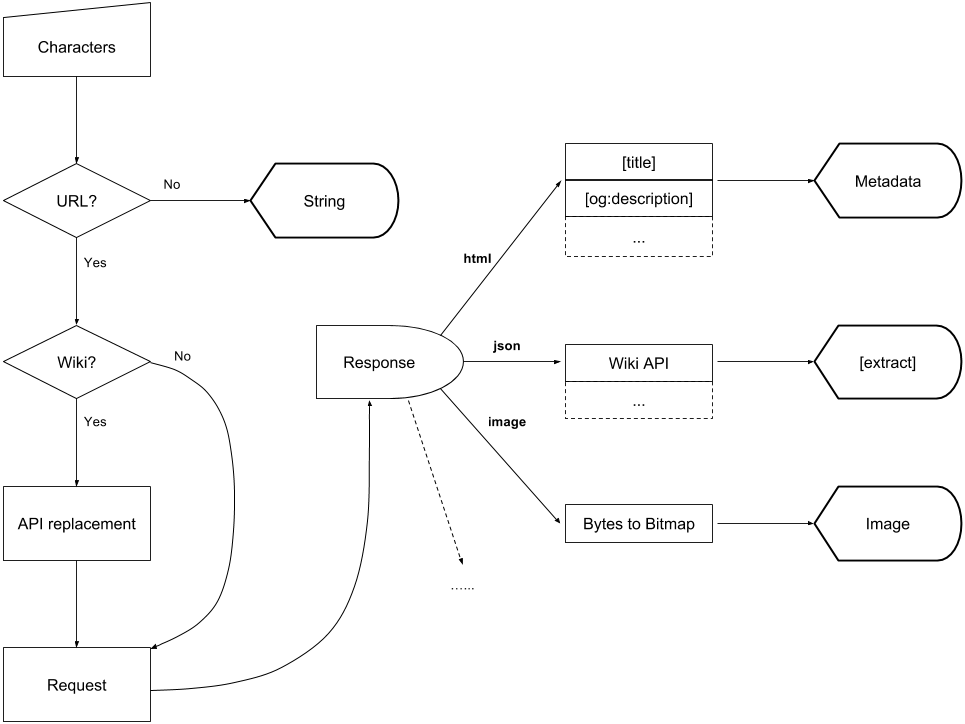
\includegraphics[width=\linewidth]{Figures/description-analysis.png}
\decoRule
\end{figure}

In order to get an extracted content from a wikipedia page, we can transform the URL to a Wiki-API based open-search url \parencite{wiki.api.2016}, which will returns a json format raw data that we can easily get what we need from different json tags.

\[
\begin{array}{lr}
\begin{aligned}
\text{Replace}\;&\code{.wikipedia.org/wiki/}\\
\text{To}\;&\code{.wikipedia.org/w/api.php?}APIs\\
\end{aligned}
\end{array}
\]

Where $APIs$ is:

\[
\begin{array}{lr}
\begin{aligned}
\code{format=json}&\\
&\code{\&action=query}\\
&\code{\&redirects=1}\\
&\code{\&prop=extracts}\\
&\code{\&exintro=}\\
&\code{\&explaintext=}\\
&\code{\&indexpageids=}\\
&\code{\&titles=}\\
\end{aligned}
\end{array}
\]

For $html$ parser, we introduced jsoup (it is a Java library for working with real-world HTML \parencite{joup.2016}), to get the basic information we need, such as $title$, and some other metadata. In this project, I am also use $og:description$ (one of the open graph meta tags \parencite{ogp.2014}) from the html source if it exist.

%****************************************************************
\subsection{OBJ Model}

A simple and common OBJ format model can be loaded as an extra model for the placemarker.

****************************************************************\\%####
vfn\\

%****************************************************************
\section{Information Display}

A textfield is a a rectangle vertices based renderable component to display text on a flat plane. Since it is a GL scene, the actual text will be drawn as a texture. By a constant width and native \code{android.text.StaticLayout} support, the height of the texture can be calculated. 

A menu contains multi-textfield can be seen as an empty textfield based which texture is fill full a pure background color, and several  textfields are laid out on the top of it with a certain vertical dimension.

A head rotation matrix (quaternion matrix \parencite{jvv.quaternions.2013}) is required for locating object in front of camera \parencite{mathworks.quaternion-rotation.2016} .

****************************************************************\\%####
quaternions\\

%****************************************************************
\section{Camera Movement}

In general, there are two sensors can be useful to manager camera movement: ACCELEROMETER (API level 3), LINEAR\_ACCELERATION (API level 9) and STEP\_DETECTOR (API level 19). 

LINEAR\_ACCELERATION is same as ACCELERATION which measures the acceleration force in meter per second repeatedly, except linear acceleration sensor is a synthetic sensor with gravity filtered out. 

\[
\begin{array}{lr}
Linear Acceleration = Accelerometer Data - Gravity\\
v = \int a\,dt\\
x = \int v\,dt\\
\end{array}
\]

First of all, we take the acclerometer data and remove gravity that is called gravity compensation, whatever is left is linear movement. Then we have to integrate it one to get velocity, integrated again to get position, which is called double integral. Now if the first integral creates drift, double integrals are really nasty that they create horrible drift. Because of these noise, using acceleration data it isn't so accurate, it is really hard to do any kind of linear movement \parencite{GoogleTechTalks.sensor-fusion.2010}.

On the other hand, use step counter from STEP\_DETECTOR, and pedometer algorithm for pedestrian navigation, that in fact works very well for this project.

\[
\begin{array}{lr}
p_1 = p_0 + v_0 \times dt\\
v_1 = v_0 + a \times dt\\
\end{array}
\]

The accuracy of this depends on how precision we can get for changing velocity. Considering that velocity is made of 3-axis directions, the current heading direction is required for a correct velocity calculation. Since the frame life cycle is implemented based on \parencite{Google.VR-SDK.2016}, which provide the heading direction in each frame callback. So I collect everything I need from the last frame to new frame, and update both velocity and position for each new frame.

For updating process, first of all, 

First of all, damping is required. I reduce velocity by a percentage. It is simply for avoiding that camear taking too long to stop. Damping by percentage can stable and stop the camera in a certain of time that won't be affected by the current camera speed. 


Secondly, a constant value in head forwarding direction is been used as a pulse for each step. Because a step is happening instantaneously which implies $a\,dt$ made by each step is actually can be replace by a constant value.

\begin{figure}[H]
\caption[camera-movement]{Camera movement}
\label{fig:camera-movement}
\centering
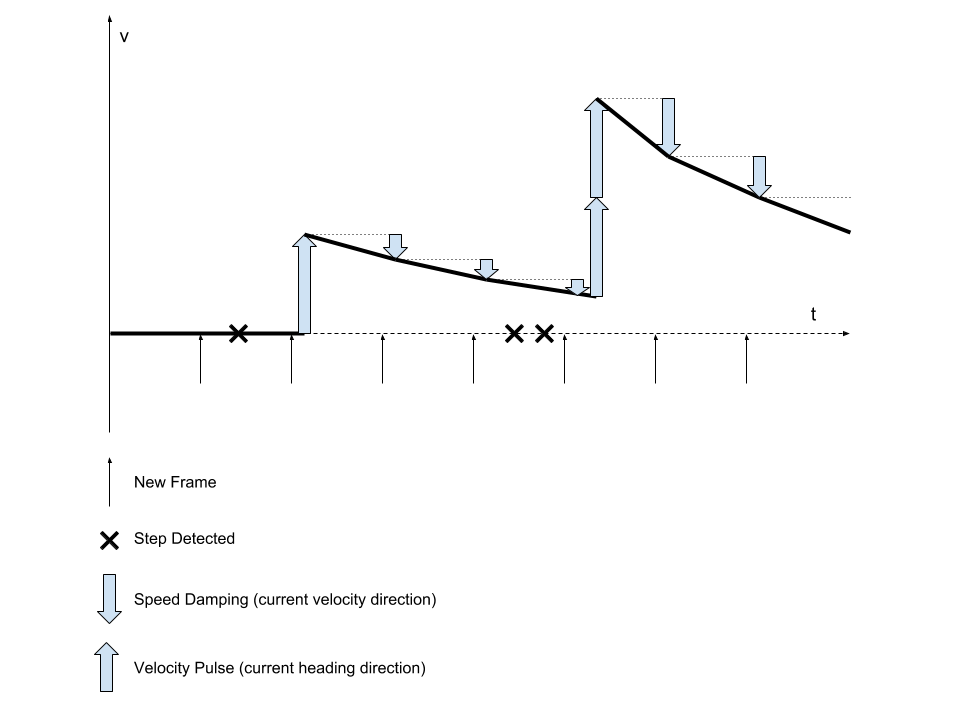
\includegraphics[width=\linewidth]{Figures/camera-movement.png}
\decoRule
\end{figure}

For each new frame:

\[
\begin{array}{lr}
\begin{aligned}
\overrightarrow{V_0} &= \overrightarrow{V_0} \cdot Damping\\
\overrightarrow{P_1} &= \overrightarrow{P_0} + \overrightarrow{V_0} \cdot dt\\
\overrightarrow{V_1} &= \overrightarrow{V_0} + \overrightarrow{Forwarding} \cdot Pulse \cdot Steps\\
Damping &\in [0,\enspace1]\\
Pulse &\in [0,\enspace \infty)\\
\end{aligned}
\end{array}
\]

%****************************************************************
\section{Ray Intersection}

Detect collisions between ray and models is the key to allow user selecting objects in the VR would, which is one of the importent experience for user interaction.

A ray can be describe in a equation with known ray start position \emph{$\overrightarrow{R_0}$} and ray direction \emph{$\overrightarrow{R_d}$}.

\begin{equation}
\label{equ:ray-t}
\overrightarrow{R(t)} = \overrightarrow{R_0} + \overrightarrow{R_d} \cdot t
\end{equation}

%****************************************************************
\subsection{Ray-Sphere}

\begin{figure}[H]
\caption[ray-sphere-intersection]{Ray-Sphere intersection}
\label{fig:ray-sphere}
\centering
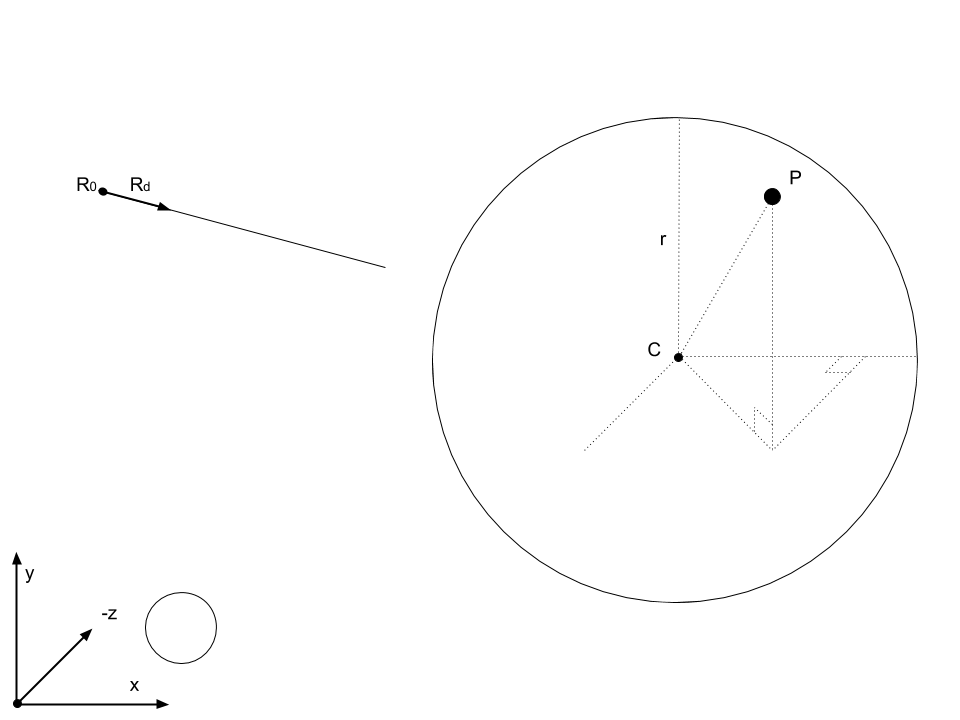
\includegraphics[width=\linewidth]{Figures/ray-sphere-intersection.png}
\decoRule
\end{figure}

A point \emph{P} on the surface of sphere should match the equation:

\begin{equation}
\label{equ:sphere-surface}
(x_p - x_c)^2 + (y_p - y_c)^2 + (z_p - z_c)^2 = r^2
\end{equation}

If the ray intersects with the sphere at any position\;\emph{P} must match the equation \ref{equ:ray-t} and \ref{equ:sphere-surface}. Therefor the solution of \emph{t} in the cointegrate equation implies whether or not the ray will intersect with the sphere:

\[
\begin{aligned}
(x_{R_0} + x_{R_d} \cdot t - x_c)^2 &+ (y_{R_0} + y_{R_d} \cdot t - y_c)^2 + (z_{R_0} + z_{R_d} \cdot t - z_c)^2 = r^2\\
&\vdots\\
x_{R_d}^2\,t^2 &+ (2\,x_{R_d}\,(x_{R_0} - x_c))\,t + (x_{R_0}^2 - 2\,x_{R_0}\,x_c + x_c^2)\\
+\;y_{R_d}^2\,t^2 &+ (2\,y_{R_d}\,(y_{R_0} - y_c))\,t + (y_{R_0}^2 - 2\,y_{R_0}\,y_c + y_c^2)\\
+\;z_{R_d}^2\,t^2 &+ (2\,z_{R_d}\,(z_{R_0} - z_c))\,t + (z_{R_0}^2 - 2\,z_{R_0}\,z_c + z_c^2) = r^2\\
\end{aligned}
\]

It can be seen as a quadratic formula:

\begin{equation}
\label{equ:sphere-surface-quadratic-formula}
a\,t^2 + b\,t + c = 0
\end{equation}

At this point, we are able to solved the \emph{t}:

\[
t =
\begin{cases}
\frac{-b \pm \sqrt{b^2 - 4\,a\,c}}{2\,a} & \text{if }\;b^2 - 4\,a\,c > 0\\
\frac{-b}{2\,a} & \text{if }\; b^2 - 4\,a\,c = 0\\
\varnothing & \text{if }\; b^2 - 4\,a\,c < 0\\
\end{cases}
\]

Then, I take a further step to get rid of formula complexity.

$\because$ Equation \ref{equ:sphere-surface},\,\ref{equ:sphere-surface-quadratic-formula}
\[
\begin{array}{lr}
a = x_{R_d}^2 + y_{R_d}^2 + z_{R_d}^2\\
b = 2\,(x_{R_d}\,(x_{R_0} - x_c) + y_{R_d}\,(y_{R_0} - y_c) + z_{R_d}\,(z_{R_0} - z_c))\\
c = (x_{R_0} - x_c)^2 + (y_{R_0} - y_c)^2 + (z_{R_0} - z_c)^2 - r^2\\
\end{array}
\]

$\And$
\[
\begin{array}{lr}
\begin{aligned}
\norm{\overrightarrow{R_d}} &= \sqrt{x_{R_d}^2 + y_{R_d}^2 + z_{R_d}^2} = 1\\
\overrightarrow{V_{c\_R_0}} &= \overrightarrow{R_0} - \overrightarrow{C} = \overrightarrow{(x_{R_0} - x_c,\enspace y_{R_0} - y_c,\enspace z_{R_0} - z_c)}\\
\end{aligned}
\end{array}
\]

$\therefore$
\[
\begin{array}{lr}
a =1\\
b = 2 \cdot \overrightarrow{R_d} \cdot \overrightarrow{V_{c\_R_0}}\\
c = \overrightarrow{V_{c\_R_0}} \cdot \overrightarrow{V_{c\_R_0}} \cdot r^2\\
\end{array}
\]

$\because$ The formula for \emph{t} can also be optimized
\[
\begin{array}{lr}
\frac{-b \pm \sqrt{b^2 - 4\,a\,c}}{2\,a} = -\alpha \pm \sqrt{\beta}\\
\alpha = \frac{1}{2}\,b\\
\beta = \alpha^2 - c\\
\end{array}
\]

$\therefore$ The final solution for \emph{t}
\[
t =
\begin{cases}
 -\alpha \pm \sqrt{\beta} & \text{if }\;\beta > 0\\
-\alpha & \text{if }\;\beta = 0\\
\varnothing & \text{if }\;\beta < 0\\
\end{cases}
\]

And the collision position for each \emph{t} is:

\[
\overrightarrow{P} = \overrightarrow{R_0} + \overrightarrow{R_d} \cdot t
\]

%****************************************************************
\subsection{Ray-Plane}

\begin{figure}[H]
\caption[ray-plane-intersection]{Ray-Plane intersection}
\label{fig:ray-plane}
\centering
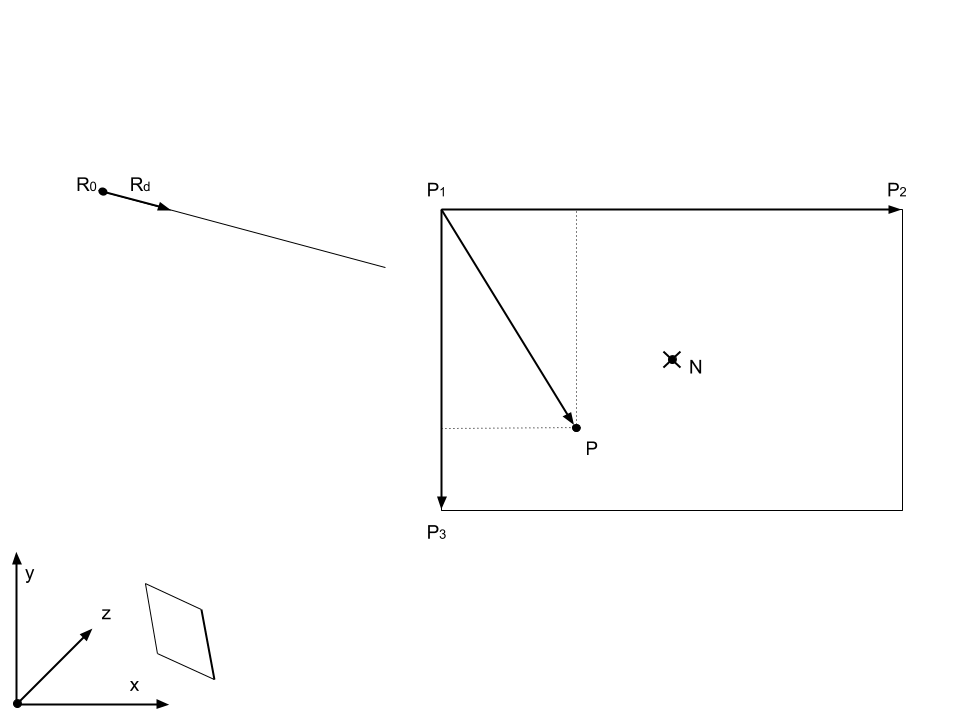
\includegraphics[width=\linewidth]{Figures/ray-plane-intersection.png}
\decoRule
\end{figure}

If a point \emph{P} on the plane and also belongs to the ray, we have quadric equation:

\begin{equation}
\label{equ:ray-plane-intersection}
\begin{array}{lr}
(\overrightarrow{P} - \overrightarrow{P_1}) \cdot \overrightarrow{N} = 0\\
\overrightarrow{P} = \overrightarrow{R_0} + \overrightarrow{R_d} \cdot t\\
\end{array}
\end{equation}

Solution for the \emph{t} is:

\[
t =
\begin{cases}
\frac{-\overrightarrow{N} \cdot (\overrightarrow{R_0} - \overrightarrow{P_1})}{\overrightarrow{N} \cdot \overrightarrow{R_d}} & \text{if }\;\overrightarrow{N} \cdot \overrightarrow{R_d} \nsim 0\\
\varnothing & \text{if }\;\overrightarrow{N} \cdot \overrightarrow{R_d} \sim 0\\
\end{cases}
\]

At last, we have to verify if the collision is inside of the quadrangle by putting \emph{t} back to \ref{equ:ray-plane-intersection}, \parencite{stackoverflow.ray-plane.2014} the \emph{t} is valid only if:\\

\[
\begin{array}{lr}
\mu = \sqrt{(\overrightarrow{P} - \overrightarrow{P_1}) \cdot (\overrightarrow{P_2} - \overrightarrow{P_1}))} \in [0,\enspace\norm{\overrightarrow{P_2} - \overrightarrow{P_1}}]\\
\nu = \sqrt{(\overrightarrow{P} - \overrightarrow{P_1}) \cdot (\overrightarrow{P_3} - \overrightarrow{P_1}))} \in [0,\enspace\norm{\overrightarrow{P_3} - \overrightarrow{P_1}}]\\
\end{array}
\]

%****************************************************************
\subsection{Ray-Box}
% \parencite{scratchapixel.ray-plane-3d} 
% \parencite{Williams.ray-box.2005}

There is a octree implementation \ref{section:octree} in the VR 3D world that separate the 3D world to invisible 3D boxes that each box contains a certain number of other models. It is to avoid unnecessary ray-object collision detection. In this section, I am going to first explain Ray-Box-2D collision detection \parencite{Tavian.ray-box-2d.2011}, then derive out Ray-Box-3D intersection.

%****************************************************************
\subsubsection{Ray-Box-2D}

\begin{figure}[H]
\caption[ray-box-2d-intersection]{Ray-Box-2D intersection}
\label{fig:ray-box-2d}
\centering
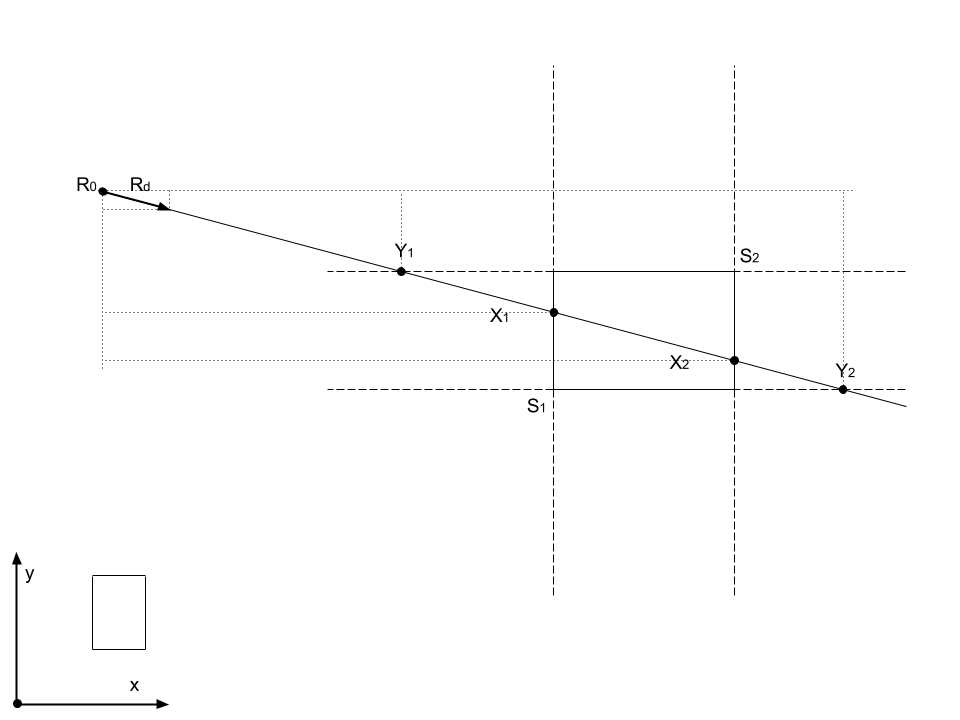
\includegraphics[width=\linewidth]{Figures/ray-box-2d-intersection.png}
\decoRule
\end{figure}

$\because$ Known $R_0$,\enspace$R_d$,\enspace$P_1$,\enspace$P_2$
\begin{multicols}{2}
\noindent
\[
X_1 =
\begin{cases}
x_{P_1} - x_{R_0} & \text{if }\;x_{R_d} > 0\\
x_{P_2} - x_{R_0} & \text{if }\;x_{R_d} < 0\\
\end{cases}
\]
\[
X_2 =
\begin{cases}
x_{P_2} - x_{R_0} & \text{if }\;x_{R_d} > 0\\
x_{P_1} - x_{R_0} & \text{if }\;x_{R_d} < 0\\
\end{cases}
\]
\[
\begin{array}{lr}
t_{X_1} = \frac{X_1}{x_{R_d}}\\
t_{X_2} = \frac{X_2}{x_{R_d}}\\
\end{array}
\]
\columnbreak
\[
Y_1 =
\begin{cases}
y_{P_1} - y_{R_0} & \text{if }\;y_{R_d} > 0\\
y_{P_2} - y_{R_0} & \text{if }\;y_{R_d} < 0\\
\end{cases}
\]
\[
Y_2 =
\begin{cases}
y_{P_2} - y_{R_0} & \text{if }\;y_{R_d} > 0\\
y_{P_1} - y_{R_0} & \text{if }\;y_{R_d} < 0\\
\end{cases}
\]
\[
\begin{array}{lr}
t_{Y_1} = \frac{Y_1}{y_{R_d}}\\
t_{Y_2} = \frac{Y_2}{y_{R_d}}\\
\end{array}
\]
\end{multicols}

$\And$ When collision happens,  we have formula:
\[
\begin{array}{lr}
\begin{aligned}
t_{X_1} &< t_{X_2}\\
t_{Y_1} &< t_{Y_2}\\
\end{aligned}
\end{array}
\]

$\therefore$ Which is
\begin{equation}
\label{equ:ray-box-2d-intersection}
max(t_{X_1},\enspace t_{Y_1}) < min(t_{X_2},\enspace t_{Y_2})
\end{equation}

%****************************************************************
\subsubsection{Ray-Box-3D}

\begin{figure}[H]
\caption[ray-box-3d-intersection]{Ray-Box-3D intersection}
\label{fig:ray-box-3d}
\centering
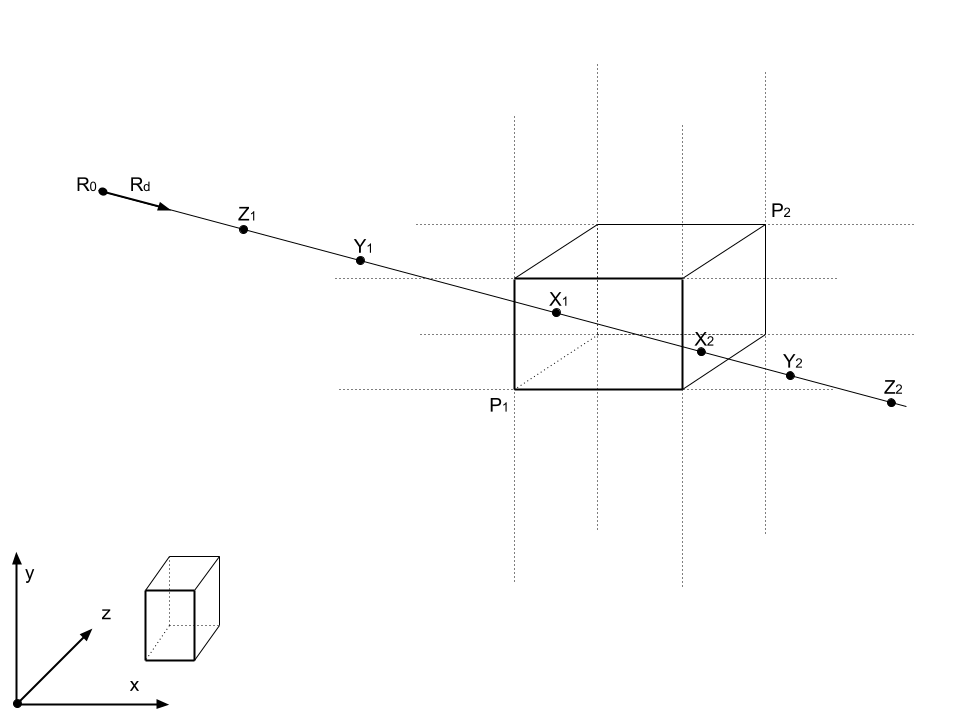
\includegraphics[width=\linewidth]{Figures/ray-box-3d-intersection.png}
\decoRule
\end{figure}

$\because$ Known $R_0$,\enspace$R_d$,\enspace$P_1$,\enspace$P_2$
\begin{multicols}{2}
\noindent
\[
X_1 =
\begin{cases}
x_{P_1} - x_{R_0} & \text{if }\;x_{R_d} > 0\\
x_{P_2} - x_{R_0} & \text{if }\;x_{R_d} < 0\\
\end{cases}
\]
\[
X_2 =
\begin{cases}
x_{P_2} - x_{R_0} & \text{if }\;x_{R_d} > 0\\
x_{P_1} - x_{R_0} & \text{if }\;x_{R_d} < 0\\
\end{cases}
\]
\[
\begin{array}{lr}
t_{X_1} = \frac{X_1}{x_{R_d}}\\
t_{X_2} = \frac{X_2}{x_{R_d}}\\
\end{array}
\]
\columnbreak
\[
Y_1 =
\begin{cases}
y_{P_1} - y_{R_0} & \text{if }\;y_{R_d} > 0\\
y_{P_2} - y_{R_0} & \text{if }\;y_{R_d} < 0\\
\end{cases}
\]
\[
Y_2 =
\begin{cases}
y_{P_2} - y_{R_0} & \text{if }\;y_{R_d} > 0\\
y_{P_1} - y_{R_0} & \text{if }\;y_{R_d} < 0\\
\end{cases}
\]
\[
\begin{array}{lr}
t_{Y_1} = \frac{Y_1}{y_{R_d}}\\
t_{Y_2} = \frac{Y_2}{y_{R_d}}\\
\end{array}
\]
\end{multicols}
\begin{multicols}{2}
\noindent
\[
Z_1 =
\begin{cases}
z_{P_1} - z_{R_0} & \text{if }\;z_{R_d} > 0\\
z_{P_2} - z_{R_0} & \text{if }\;z_{R_d} < 0\\
\end{cases}
\]
\[
Z_2 =
\begin{cases}
z_{P_2} - z_{R_0} & \text{if }\;z_{R_d} > 0\\
z_{P_1} - z_{R_0} & \text{if }\;z_{R_d} < 0\\
\end{cases}
\]
\[
\begin{array}{lr}
t_{Z_1} = \frac{Z_1}{z_{R_d}}\\
t_{Z_2} = \frac{Z_2}{z_{R_d}}\\
\end{array}
\]
\columnbreak
\[
\]
\end{multicols}

$\And$ When collision happens,  we have formula:
\[
\left\{
\begin{array}{lr}
\begin{aligned}
t_{X_1} &< t_{X_2}\\
t_{Y_1} &< t_{Y_2}\\
t_{Z_1} &< t_{Z_2}\\
\end{aligned}
\end{array}
\right.
\]

$\therefore$ Which is
\begin{equation}
\label{equ:ray-box-3d-intersection}
max(t_{X_1},\enspace t_{Y_1},\enspace t_{Z_1}) < min(t_{X_2},\enspace t_{Y_2},\enspace t_{Z_2})
\end{equation}

%****************************************************************
